\documentclass[10pt]{beamer}

%%%
% PREAMBLE FOR THIS DOC 
%%%
%https://tex.stackexchange.com/questions/68821/is-it-possible-to-create-a-latex-preamble-header
\usepackage{/Users/miw267/Repos/csci246_spring2025/slides/preambles/beamer_preamble_for_CSCI246}


\usepackage{bm}


%%% TRY TO RESHOW TOC AT EACH SECTION START (with current section highlighted)
% Reference: https://tex.stackexchange.com/questions/280436/how-to-highlight-a-specific-section-in-beamer-toc
\newcommand\tocforsect[2]{%
  \begingroup
  \edef\safesection{\thesection}
  \setcounter{section}{#1}
  \tableofcontents[#2,currentsection]
  \setcounter{section}{\safesection}
  \endgroup
}


%%%% HERES HOW TO DO IT CORRECTLY
% FIRST IN .STY FILE, DO
%\usetheme[sectionpage=none]{metropolis}
% THEN AT EACH SECTION DO
%\begin{frame}{Outline}
%  \tableofcontents[currentsection]	
%\end{frame}



%\setbeamertemplate{navigation symbols}{}
%\setbeamertemplate{footline}[frame number]{}


%%%
% DOCUMENT
%%%

\begin{document}

%\maketitle

%% Title page frame
%\begin{frame}
%    \titlepage 
%\end{frame}



\title{04/04/2025: Big O Notation}
\author{CSCI 246: Discrete Structures}
\date{Textbook reference: Sec 7.2, Ponomarenko}

\begin{frame}
    \titlepage 
\end{frame}


\begin{frame}
\small
\begin{mygreenbox}[title=Graded Quiz Pickup]
Quizzes are in the front of the room, grouped into four bins (A-G, H-L, M-R, S-Z) by last name. The quizzes are upside down with your last name on the back. Come find yours before, during, or after class. Only turn the quiz over if it's yours.
\end{mygreenbox} 
\vfill 
%\begin{myredbox}[title=Friday's Problems Quiz]
%The problems quiz on Friday (04/02) will cover:
%\begin{itemize}
%\item Conditional Probability and Independence
%\item Random Variables
%\item Expectations	
%\end{itemize}
%
%\end{myredbox}
\vfill 
\begin{myyellowbox}[title=Today's Agenda]
\begin{itemize}
	\item Reading and problems quizzes (15 mins)
	\item Mini-lecture ($\approx$ 15 mins)
	\item Group exercises ($\approx$ 15 mins)
\end{itemize}


\end{myyellowbox}
\vfill 

\end{frame}






\begin{frame}[standout]
Feedback on Wednesday's Quiz
\end{frame}

\begin{frame}{Reading Quiz Scores (Extra Credit)}
\begin{figure}[ht]
        \centering
        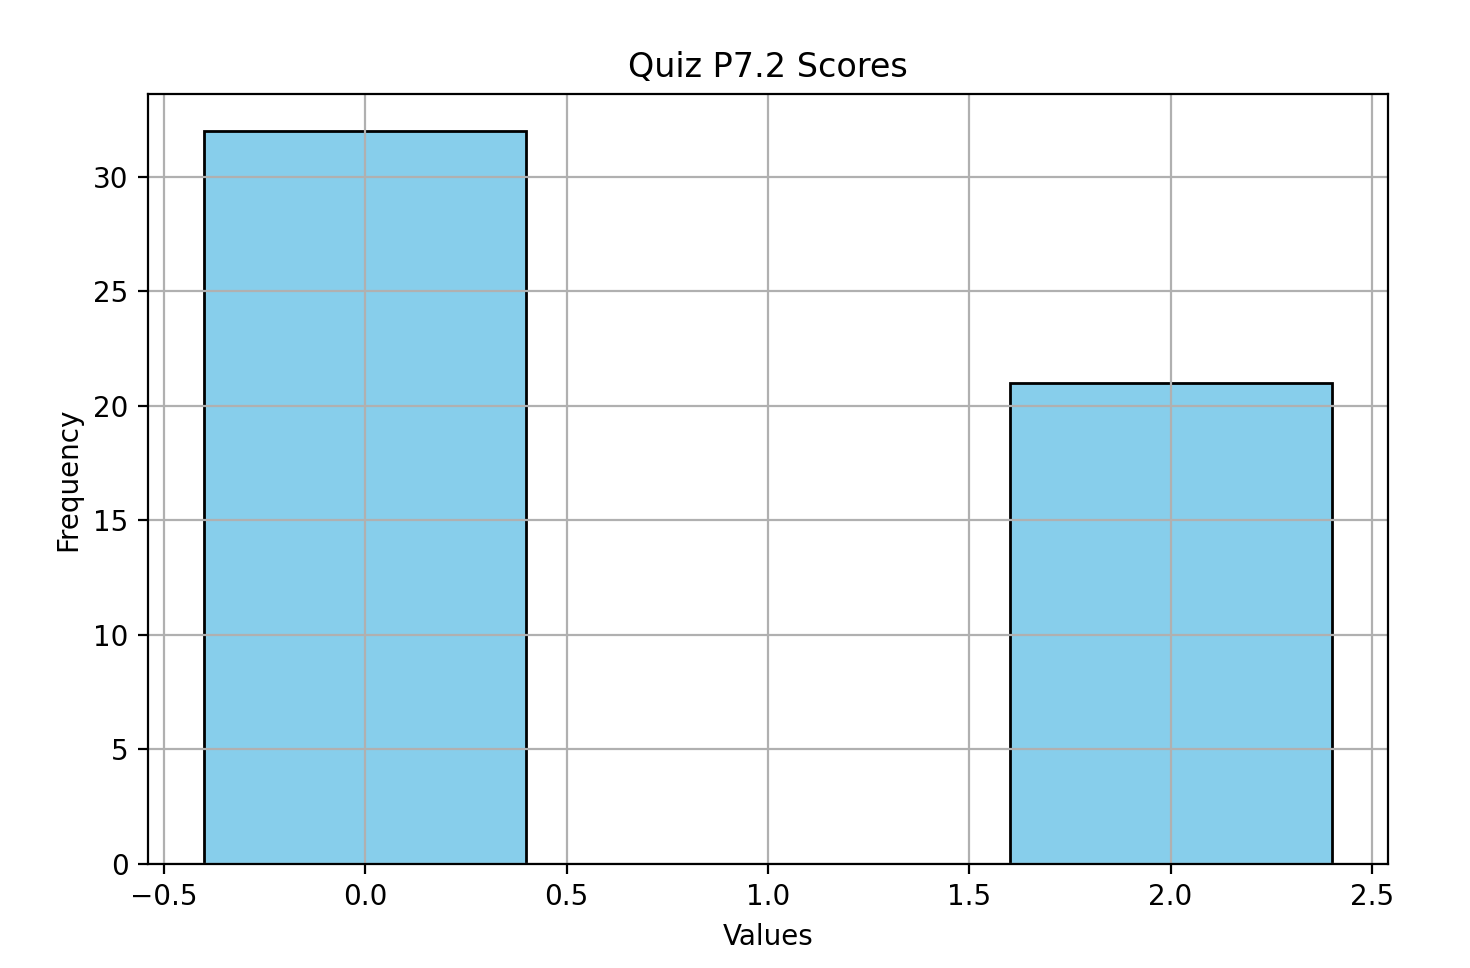
\includegraphics[width=.7\textwidth]{images/reading_quiz_scores}
   		 \caption{Median Score = 0 points extra credit}
\end{figure}
\vfill 
\textbf{Grading Rubric:}  2 points extra credit for perfect answer.
\end{frame}	


%\begin{frame}[standout]
%Reading quiz.
%\end{frame}
%
%\begin{frame}
%\begin{myyellowbox}[title=Reading Quiz (Big O notation)]
%Consider the sequence $a_n = 3n + 100$.  Prove that $a_n = \Omega(n)$. 
%\end{myyellowbox}
%\vfill 
%
%When answering the reading quiz, please use the definition below. 
%\vfill
%
%\begin{mygreenbox}[title=\text{Definition 7.11 from Ponomarenko}]
%Given a sequence $a_n$ and a test sequence $b_n$, we say that \enquote{$a_n$ is big Omega of $b_n$}, writing $a_n = \Omega(b_n)$, to mean: There is some $n_0 \in \mathbb{N}$ and some $M \in \R$ such that for every $n \geq n_0$, we have $M|a_n| \geq |b_n|$.
%\end{mygreenbox} 
%\vfill 
%\begin{myredbox}[title=Remark]
%We can interpret $a_n = \Omega(b_n)$ to mean that the sequence $a_n$ eventually grows at least as fast as $b_n$.
%\end{myredbox}
%
%\end{frame}


\begin{frame}[standout]
Today's quiz
\end{frame}

\begin{frame}

\begin{mygreenbox}[title=\text{Problems Quiz (Conditional Prob, Random Variables, Expectation)}]
\begin{enumerate}
	\item Let $(S,P)$ be the sample space with $S=\set{1,2,\hdots, 10}$ and $P(x) =\frac{1}{10}$ for all $x \in S$.  Let $A$ be the event \enquote{is even} and $B$ be the event \enquote{is prime}. Calculate $P(A \cond B)$ and $P(B \cond A)$. Show your work.
	\item Two cards are drawn at random (without replacement) from a standard deck of 52 cards. Let $X$ be the rank of the first card and $Y$ be the rank of the second card. Are $X$ and $Y$ independent? Justify your answer with a mathematical argument.
\end{enumerate}
\end{mygreenbox}
\vfill 
\begin{myredbox}[title=Reading Quiz (Big O notation)]
Consider the sequences $a_n = 3n + 100$ and $b_n=n$.  Show  that $a_n = O(b_n)$.  That is, show that there is some $n_0 \in \mathbb{N}$ and some $M \in \R$ such that for every $n \geq n_0$, we have $|a_n| \leq M|b_n|$.
\end{myredbox}
\end{frame}




\begin{frame}[standout]
Thoughts On Big O Notation
\end{frame}

\begin{frame}{How to compare the efficiency of algorithms?}
\begin{figure}
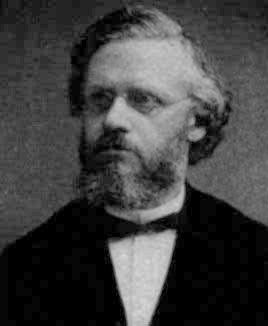
\includegraphics[width=.5\textwidth]{images/paul_bachmann}
\caption{German mathematician Paul Bachmann}

\pause 
% TikZ overlay for precise positioning
\begin{tikzpicture}[remember picture, overlay]
    \node[draw, fill=pink, rounded corners, cloud callout,  scale=0.7, font=\large, callout relative pointer={(0.5,-0.5)}] 
        at ([xshift=3.5cm,yshift=7cm]current page.south west) {Big O notation!};
\end{tikzpicture}
    
\end{figure}
\end{frame}



\begin{frame}
\small 
\begin{mygreenbox}[title=Definition]
Let $f$ and $g$ be real-valued non-negative functions defined on the same set of nonnegative integers. \\

Then $f$ is of order at most $g$, written \textbf{$\bm{f(n)}$ is $\bm{O(g(n))}$} ($f$ of $n$ is big-O of $g$ of $n$) if and only if there exist positive real number $B$ and integer $b$ such that
\[  |f(n)| \leq B |g(n)| \quad \text{for every integer } n \geq b\]	
\end{mygreenbox}
\vfill 
\begin{figure}
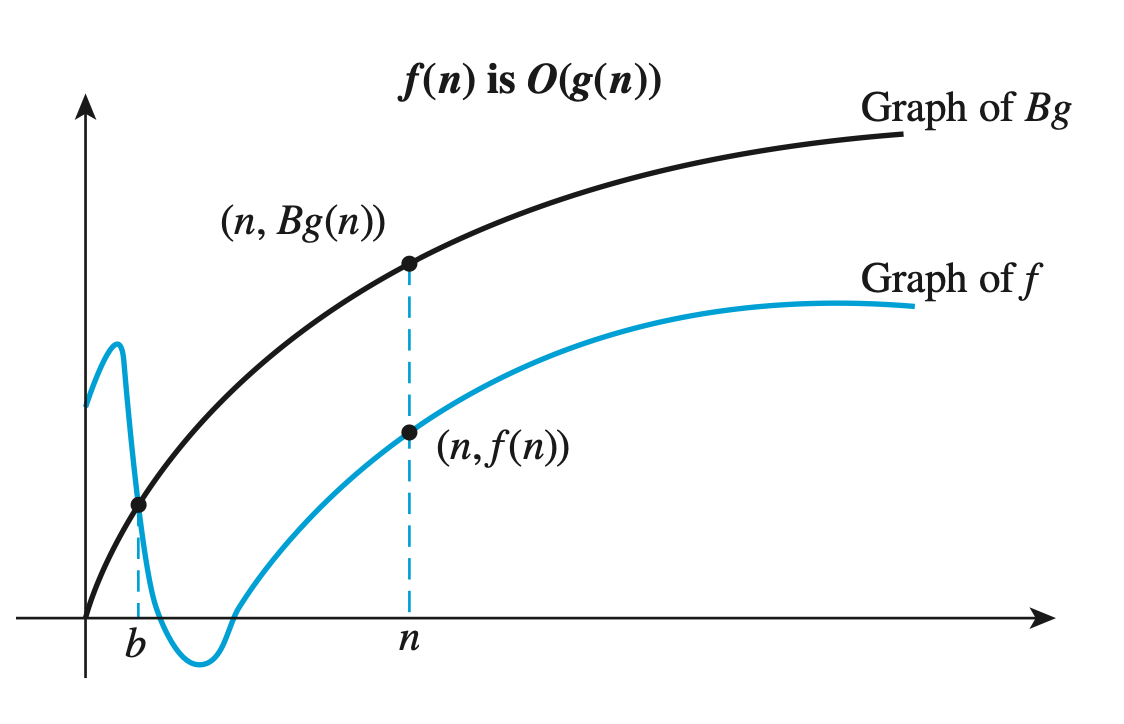
\includegraphics[width=.6\textwidth]{images/big_O.png}
\end{figure}
\pause \vfill 
\colorbox{yellow!30}{\textbf{Poll.}} How would you summarize this definition in words?
\end{frame}

\begin{frame}

\onslide+<1-> \colorbox{yellow!30}{\textbf{Poll.}} How would you summarize this definition in words?
\vfill 
\onslide+<2-> \colorbox{green!30}{\textbf{Solution.}}
The values of $f$ are  \alert<4->{eventually} less than those of a \alert<4->{positive multiple} of $g$.  \\
\vfill 
\onslide+<3->  We say that \enquote{$f$ is of order at most $g$}.
\vfill 
\onslide+<5->
\colorbox{yellow!30}{\textbf{Poll.}} What's the deal with the highlighted words (especially \alert{positive multiple})?
\end{frame}


\begin{frame}{Classification Theorem}
\footnotesize 
\begin{center}
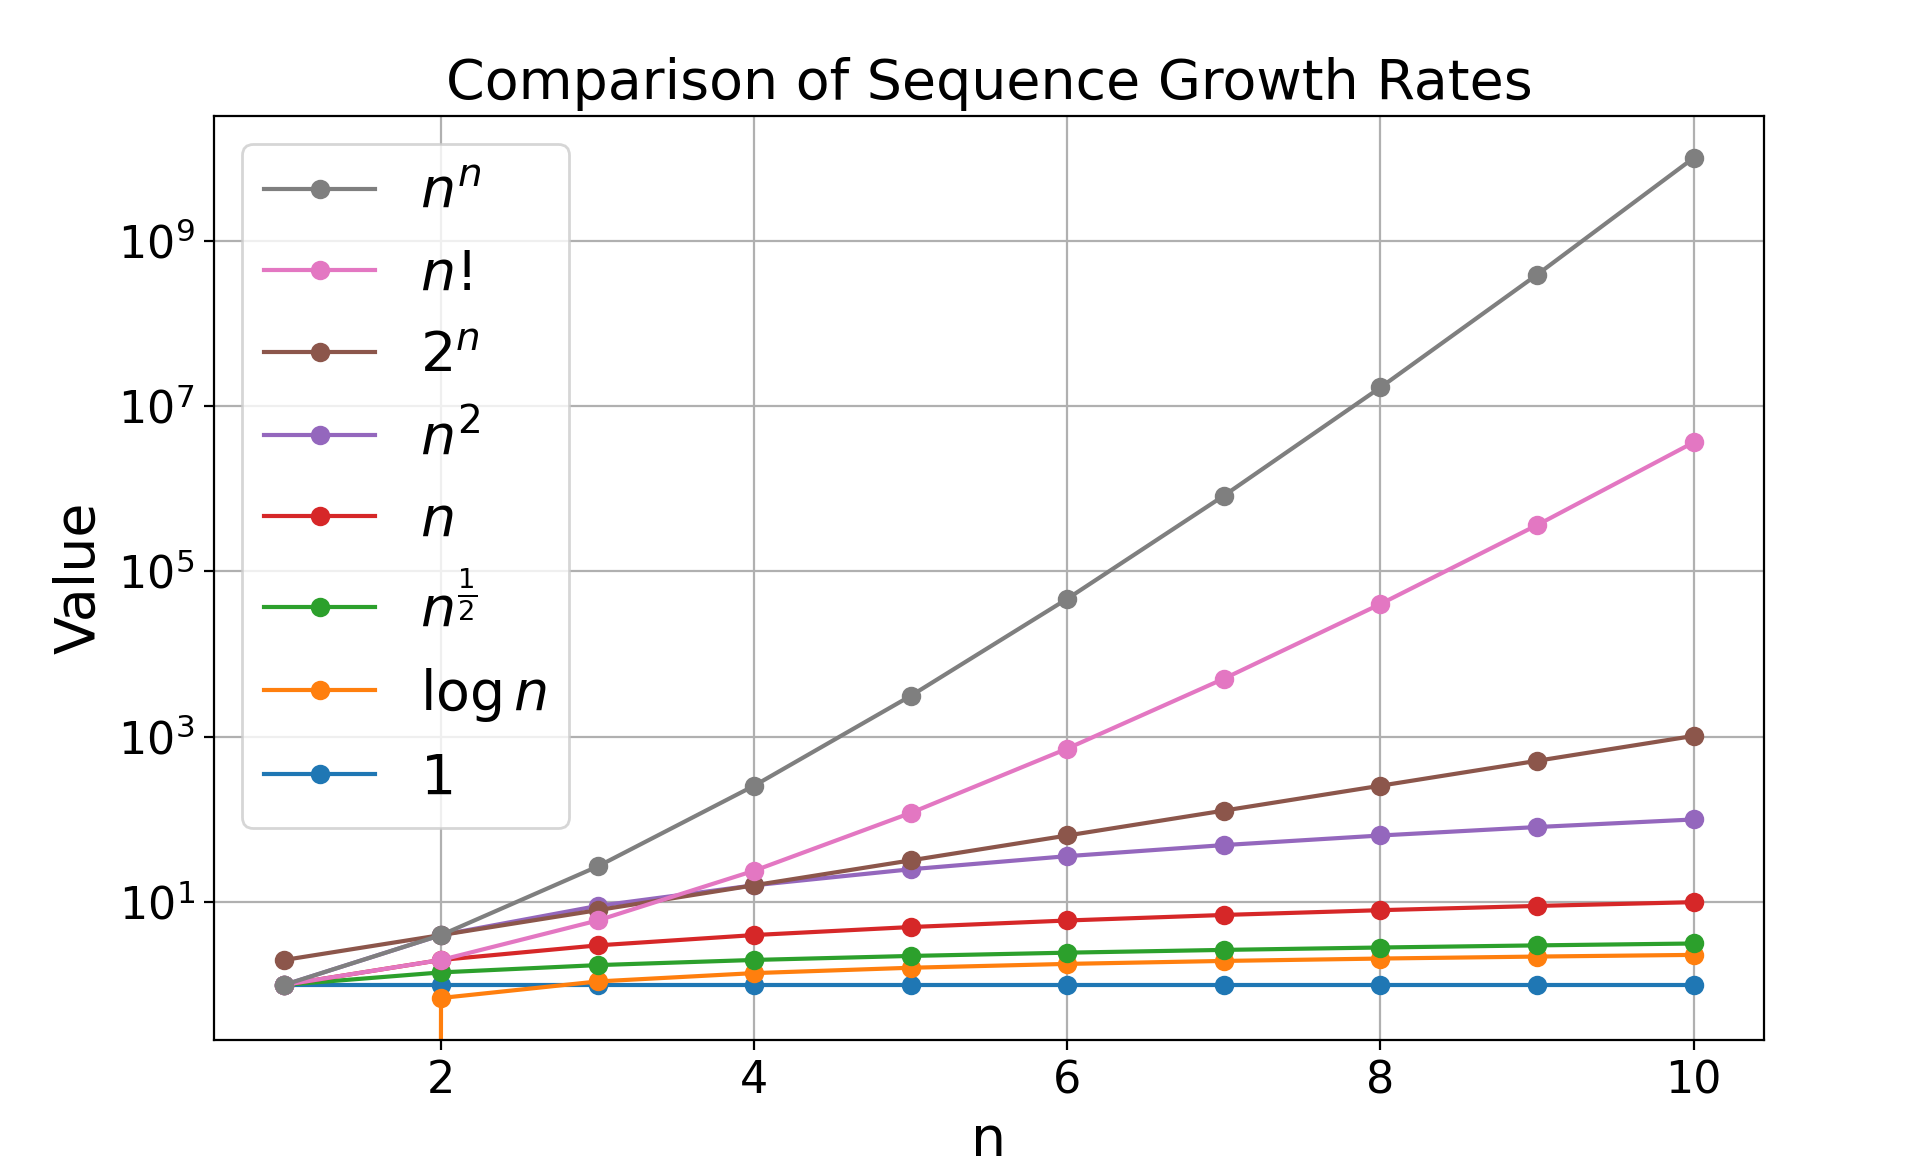
\includegraphics[width=0.7\textwidth]{images/classification_theorem.png}
\end{center}
\vfill 
\colorbox{yellow!30}{\textbf{Poll.}} How should we interpret this graph?
\vfill \pause 
\begin{itemize}
\item A taxonomy of growth rates (or scaling behavior): Any function is big O of everything equal to or above it, but is \textbf{not} big O of anything below it. \pause 
\item \textbf{Example}:  \colorbox{red!30}{$n$} is big O of \colorbox{red!30}{$n$}, \colorbox{purple!30}{$n^2$}, \colorbox{brown!30}{$2^n$}, \colorbox{pink!30}{$n!$}, and \colorbox{gray!30}{$n^n$}.  Even if we multiply  \colorbox{red!30}{$n$}  by a large constant, those functions will always eventually get bigger! \pause 
\item \textbf{Anti-Example}:  \colorbox{red!30}{$n$} is not big O of \colorbox{green!30}{$n^{\half}$}.  No matter how much you scale up \colorbox{green!30}{$n^{\half}$} by a large constant,  \colorbox{red!30}{$n$} will eventually get bigger!
\end{itemize}

\end{frame}





\begin{frame}{How to check Big O membership?}
\footnotesize 

\begin{mygreenbox}[title=\text{Example: $f(n) = 3n+100$ is $O(n)$}]
\textbf{Proof.} Take $n \geq 1$. Then 
\[ |3n+100| \leq  |3n+100n| = 103|n|.\]
\hfill (To satisfy the definition of big O, we take $b=1, B=103$.)
\end{mygreenbox}
\vspace{-.1cm}
\vfill 
\pause 
\begin{mygreenbox}[title=\text{Example: $f(n) = 9n^2+3n-2$ is $O(n^2)$.}]
\textbf{Proof.} Take $n \geq 1$. Then 
\[ |9n^2+3n-2| \leq  |9n^2+3n^2+2n^2| = 14|n^2|.\]
\hfill (To satisfy the definition of big O, we take $b=1, B=14$.)
\end{mygreenbox}
\small 
\vfill \pause 
\colorbox{red!30}{\textbf{Remark.}} Big O notation hides irrelevant details.
\vfill \pause 
\colorbox{yellow!30}{\textbf{Poll.}} Do you see a pattern?
\vfill \pause 
\colorbox{green!30}{\textbf{Solution.}} Polynomials are big O of their highest-order term.
\vfill \pause 
\colorbox{red!30}{\textbf{Remark.}} ...and also big O of still higher-order terms.   E.g. for $n \geq 1$,
\vspace{-.1cm}
\[14|n^2| \leq 14|n^3| \leq 14|n^4| \leq \hdots \]
\end{frame}



\begin{frame}{Classification Theorem: Zooming In On Polynomials}
\small 
\begin{center}
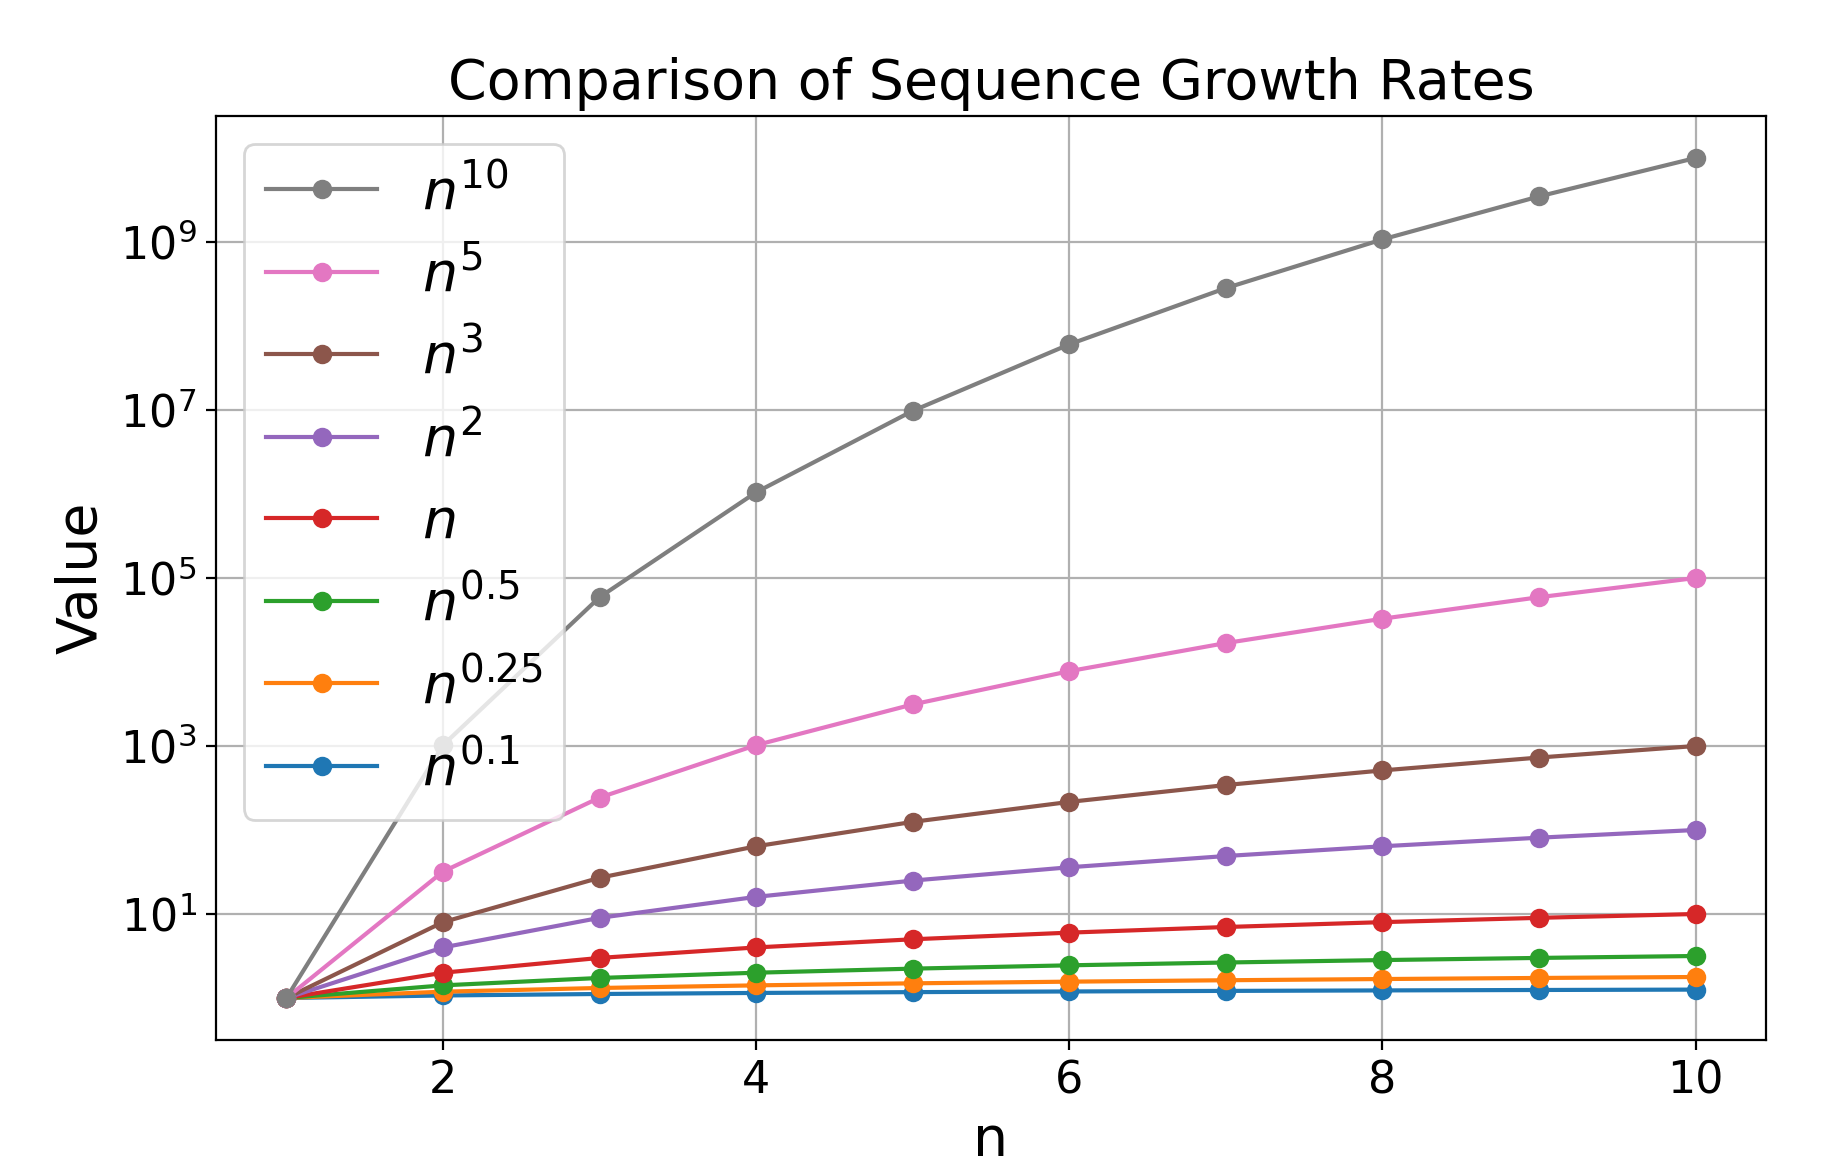
\includegraphics[width=0.65\textwidth]{images/big_O_polynomials.png}
\end{center}
\vfill 
\pause 
A taxonomy of growth rates: As you go down the legend, each function is big O of everything above it, but \textbf{not} big O of everything below it. \pause 
\vfill \pause 
\begin{myredbox}[title=Theorem]
For any function $f$ and positive real numbers $u$ and $v$ with $u<v$,
\[f \text{ is } O(x^u) \implies  f \text{ is } O(x^v)\]
\end{myredbox}

\end{frame}

\begin{frame}{A major problem with Big O statements}

\onslide+<1->
\colorbox{yellow!30}{\textbf{Poll.}} Suppose a person is analyzing the efficiency of algorithms, and finds that $f \text{ is } O(x^5)$ and $g \text{ is } O(x^4)$.  Because $4<5$, this person concludes that $g$ has a better algorithmic efficiency than $f$. Is this person's conclusion correct?
\vfill 

\onslide+<2->
\colorbox{green!30}{\textbf{Solution.}} No.  For instance, take $f(x) = x^2$ and $g(x)=x^3$. Then \\
\qquad \alert<3->{f}  \; is \; $O(x^2), O(x^3), O(x^4)$, \alert<3->{$O(x^5)$}, $\hdots$   \\ 
and  \\
\qquad \alert<3->{g}  \; is \;  $O(x^3)$, \alert<3->{$O(x^4)$}, $O(x^5)$, $\hdots$  \\
\vfill 
\onslide+<4->

\colorbox{red!30}{\textbf{Remark.}} The problem is that the upper bounds for Big O can be needlessly large! 

\vfill 
\onslide+<5->
 
We should interpret \enquote{$g \text{ is } O(x^4)$} as: \enquote{$g$ is of order \textbf{at most} $x^4$}.

\end{frame}


\begin{frame}{How to compare the efficiency of algorithms?}
\begin{figure}
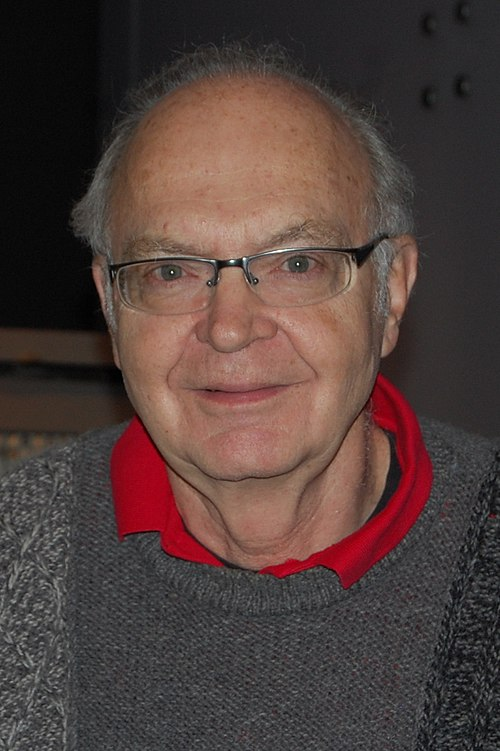
\includegraphics[width=.4\textwidth]{images/donald_knuth}
\caption{American computer scientist and mathematician Donald Knuth}

\pause 
% TikZ overlay for precise positioning
\begin{tikzpicture}[remember picture, overlay]
    \node[draw, fill=pink, rounded corners, cloud callout,  scale=0.7, font=\large, callout relative pointer={(0.5,-0.5)}] 
        at ([xshift=3.0cm,yshift=7.2cm]current page.south west) {Big Theta notation!};
\end{tikzpicture}
    
\end{figure}
\end{frame}

\begin{frame}
\small 

\begin{tabularx}{\textwidth}{c @{\hspace{0.25cm}} c @{\hspace{0.25cm}} c @{\hspace{0.25cm}} X}
\midrule 
\textbf{Big O} & $f \text{ is } O(g)$ & $f$ is of order \alert{at most} $g$  & The values of $f$ are  eventually \textbf{less} than those of a positive multiple of $g$. \\
 \vspace{.2cm}
\textbf{Big Omega} &  $f \text{ is } \Omega(g)$ & $f$ is of order \alert{at least} $g$  & The values of $f$ are  eventually \textbf{greater} than those of a positive multiple of $g$. \\
  \vspace{.2cm}
\textbf{Big Theta} &  $f \text{ is } \Theta(g)$ & $f$ is of order $g$ & The values of $f$ are  eventually \textbf{less} than those of a positive multiple of $g$ and  \textbf{greater} than those of a positive multiple of $g$.\\
\bottomrule
\end{tabularx}


	
\end{frame}



\begin{frame}
\begin{figure}
\includegraphics[width=\textwidth]{images/big_theta}
\end{figure}
\end{frame}

\begin{frame}

\begin{myredbox}[title=\text{Theorem: On Polynomial Orders}]
If $m$ is any integer with $m \geq 0$ and $c_0, c_1, c_2, \hdots c_m$ are real numbers with $c_m \geq 0$, then
\[c_m x^m + c_{m-1} x^{m-1} + \hdots + c_1 x + c_0 \text{ is } \Theta(x^m). \]
\end{myredbox}

\end{frame}




\begin{frame}[standout]
Group exercises
\end{frame}

\begin{frame}
\footnotesize 
\vfill 
\begin{columns}
\begin{column}{0.33\textwidth}
aaron.loomis: 15 \\ 
adam.wyszynski: 13 \\ 
alexander.goetz: 2 \\ 
alexander.knutson: 3 \\ 
anthony.mann: 17 \\ 
blake.leone: 19 \\ 
bridger.voss: 19 \\ 
caitlin.hermanson: 15 \\ 
cameron.wittrock: 4 \\ 
carsten.brooks: 7 \\ 
carver.wambold: 8 \\ 
colter.huber: 16 \\ 
conner.reed1: 12 \\ 
connor.mizner: 6 \\ 
connor.yetter: 21 \\ 
derek.price4: 14 \\ 
devon.maurer: 2 \\ 
emmeri.grooms: 4 \\ 
erik.moore3: 3 \\ 
ethan.johnson18: 8 \\ 
evan.barth: 1 \\\end{column}
\begin{column}{0.33\textwidth}
evan.schoening: 9 \\ 
griffin.short: 14 \\ 
jack.fry: 10 \\ 
jacob.ketola: 11 \\ 
jacob.ruiz1: 17 \\ 
jacob.shepherd1: 4 \\ 
jada.zorn: 13 \\ 
jakob.kominsky: 12 \\ 
james.brubaker: 10 \\ 
jeremiah.mackey: 18 \\ 
jett.girard: 21 \\ 
john.fotheringham: 5 \\ 
jonas.zeiler: 1 \\ 
joseph.mergenthaler: 9 \\ 
joseph.triem: 12 \\ 
julia.larsen: 10 \\ 
justice.mosso: 16 \\ 
kaden.price: 13 \\ 
lucas.jones6: 15 \\ 
luka.derry: 17 \\ 
luke.donaldson1: 7 \\\end{column}
\begin{column}{0.33\textwidth}
lynsey.read: 14 \\ 
mason.barnocky: 11 \\ 
matthew.nagel: 1 \\ 
micaylyn.parker: 6 \\ 
michael.oswald: 20 \\ 
nolan.scott1: 19 \\ 
owen.obrien: 11 \\ 
pendleton.johnston: 2 \\ 
peter.buckley1: 6 \\ 
reid.pickert: 18 \\ 
ryan.barrett2: 3 \\ 
samuel.hemmen: 20 \\ 
samuel.mosier: 9 \\ 
samuel.rollins: 20 \\ 
sarah.periolat: 8 \\ 
timothy.true: 16 \\ 
tristan.nogacki: 5 \\ 
tyler.broesel: 18 \\ 
william.elder1: 21 \\ 
yebin.wallace: 7 \\ 
zeke.baumann: 5 \\\end{column}
\end{columns}
\vfill
\end{frame}

\begin{frame}{Group exercises}
\colorbox{green!30}{\textbf{Exercises.}}
\begin{enumerate}
	\item  Let $a_n = 1,000,000n + 3,000,000$. Prove that $a_n = O(n)$.
	\item Let $a_n = 5 + \frac{1}{n} + \frac{1}{n+1}$. Prove that $a_n = O(1)$.
	\item Let $a_n = n^2 + n + 1 + \frac{1}{n} + \sin n$. Prove that $a_n = O(n^2)$.
	\item Let $a_n = 3n^2 + 7$. Prove that $a_n = \Theta (n^2)$.
	\item Prove Theorem 7.9 from the Ponomarenko reading. 
\end{enumerate}

\vfill
\colorbox{red!30}{\textbf{Theorem 7.9 (Ponomarenko).}} Let $a_n$ be a sequence, and $b_n,c_n$ be test sequences.  If $a_n = O(b_n)$ and $b_n = O(c_n)$, then $a_n = O(c_n)$.
\end{frame}


\end{document}
